
\question{Quelle méthode de tri vous semble la mieux adaptée au tri du classement général ?}

La méthode par insertion qui semble naïve est sans doute adaptée ici car les listes triées n'évolueront peu d'une étape à l'autre et dans ce cas la méthode peut s'approcher d'une complexité linéaire.

\question{Modifier un algorithme de tri au choix pour pouvoir trier la liste obtenue en sortie de la fonction \texttt{ajoutTemps(L1,L2)} selon la dernière colonne. On l'appellera \texttt{tri$\_$modifie(liste)->list}.}


\begin{lstlisting}
####Tri par insertion modifié
def tri_insertion_modifie(T):
    n=len(T)
    for i in range(1,n):
        j=i
        v=T[i][-1]
        v2=T[i]
        while j>0 and v<T[j-1][-1]:
            T[j]=T[j-1]
            j=j-1
        T[j]=v2
    return T

####Tri rapide modifié
def partition_modifie(a,g,d):
    assert g<d
    v=a[g][-1]
    v2=a[g]
    ainf=[]
    asup=[]
    for x in a[g+1:d]:
        if x[-1]<=v:
            ainf.append(x)
        else:
            asup.append(x)
    a=a[0:g]+ainf+[v2]+asup+a[d:len(a)]
    m=len(ainf)+g
    return m,a



def tri_rapide_modifie(a,g,d):
    if g>=d-1:
        return
    else:
        m,a=partition_modifie(a,g,d)
        tri_rapide_modifie(a,g,m)
        tri_rapide_modifie(a,m+1,d)

####Tri par fusion modifié
def fusion_modifie(a0,a,g,m,d):
    i,j=g,m
    for k in range(g,d):
        if i<m and (j==d or a0[i][-1]<=a0[j][-1]):
            a[k]=a0[i]
            i=i+1
        else:
            a[k]=a0[j]
            j=j+1


def tri_fusion_modifie(a,g,d):
    a0=a[:]
    if g>=d-1:
        return
    else:
        m=(g+d)//2
        tri_fusion_modifie(a,g,m)
        tri_fusion_modifie(a,m,d)
        a0[g:d]=a[g:d]
        fusion_modifie(a0,a,g,m,d)

\end{lstlisting}



\question{Ecrire une fonction \texttt{update$\_$classement$\_$general(liste1:list,liste2:list)->list} qui à partir des deux listes du classement de l'étape 18 et du classement général renvoie la liste de la forme  \texttt{[[Nom\_1, Dossard\_1, Temps\_1], [Nom\_2, Dossard\_2, Temps\_2], ...]} triée dans l'ordre du nouveau classement général.}


\begin{lstlisting}
def update_classement_general(liste1:list,liste2:list)->list:
    LGN=ajoutTemps(LG,L18)
    sorted(LGN,key=lambda colonnes:colonnes[2])
    return LGN
\end{lstlisting}



\question{Utiliser le module \texttt{time} pour comparer les temps de traitement pour trier le classement à l'issu de la dernière étape selon votre algorithme de tri modifié et selon la fonction \texttt{sorted}.}


\begin{lstlisting}
def comparer_tri_liste(LGN,nom_de_fichier):
    temps_insertion=[]
    temps_rapide=[]
    temps_fusion=[]
    temps_sorted=[]
    for k in range(2,len(LGN)):
        LGT1=LGN[:k+1]
        LGT2=LGN[:k+1]
        LGT3=LGN[:k+1]
        LGT4=LGN[:k+1]
        tic=t.time()
        tri_fusion_modifie(LGT1,0,len(LGT1))
        toc=t.time()
        temps_fusion.append(toc-tic)
        tic=t.time()
        tri_insertion_modifie(LGT2)
        toc=t.time()
        temps_insertion.append(toc-tic)
        tic=t.time()
        tri_rapide_modifie(LGT3,0,len(LGT3))
        toc=t.time()
        temps_rapide.append(toc-tic)
        tic=t.time()
        sorted(LGT4,key=lambda colonnes:colonnes[2])
        toc=t.time()
        temps_sorted.append(toc-tic)

    plt.clf()
    plt.plot(list(range(2,len(LGN))),temps_fusion,'g-',label='fusion')
    plt.plot(list(range(2,len(LGN))),temps_rapide,'b*-',label='rapide')
    plt.plot(list(range(2,len(LGN))),temps_insertion,'r--',label='insertion')
    plt.plot(list(range(2,len(LGN))),temps_sorted,'k.-',label='sorted')
    plt.legend()
    plt.savefig(nom_de_fichier)

LGN=update_classement_general(LG,L18)
comparer_tri_liste(LGN,'tp09_durif_compare_tri1.png')
\end{lstlisting}


\begin{center}
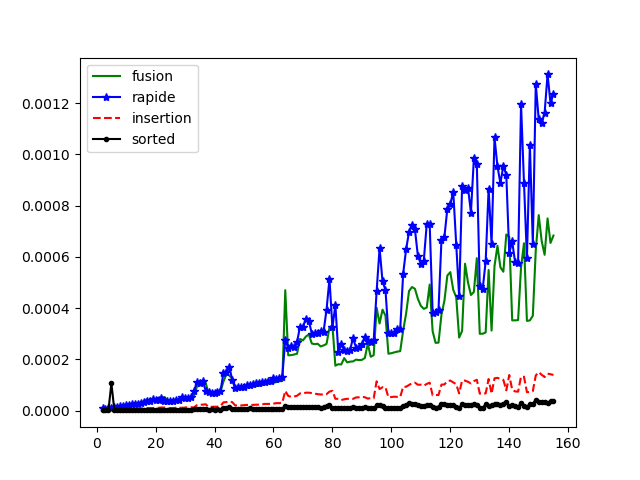
\includegraphics[width=0.5\textwidth]{programmes/tp09_durif_compare_tri1}
\end{center}

\question{Comparer les différentes méthodes de tri en traçant en fonction de la taille du tableau à traiter le temps nécessaire au tri des données. On pourra pourra pour cela utiliser un tranchage. Vous pourrez renvoyer la figure tracée à vos enseignants.}

On vérifie bien que dans ce cas la méthode par insertion est la plus adaptée.

La méthode sorted semble encore plus efficace.

\question{Facultatif : comparer les différentes méthodes de tri vues en cours appliquée sur une liste aléatoire (comme donnée précédemment) en traçant en fonction de la taille du tableau à traiter le temps nécessaire au tri des données. On pourra pourra pour cela utiliser un tranchage. Vous pourrez renvoyer la figure tracée à vos enseignants.}



Si on compare les méthodes de tri pour des listes de nombre aléatoires, voici les résultats obtenus.


\begin{center}
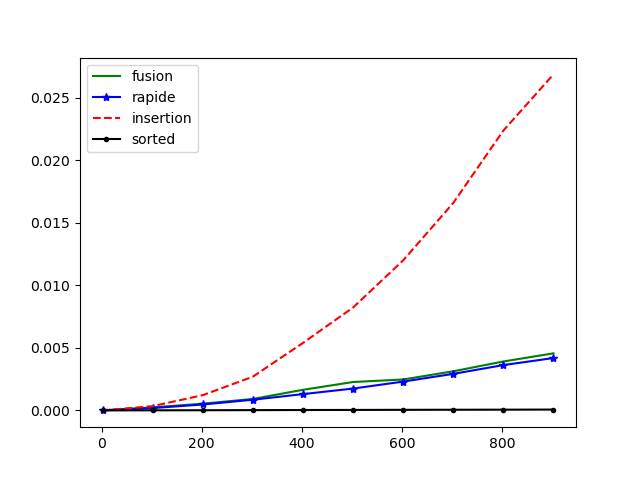
\includegraphics[width=0.5\textwidth]{programmes/tp09_durif_compare_tri2}
\end{center}



%\subsection*{Classement en cours d'étape -- Implémentation d'une file}
%On cherche à reconstituer le classement général au fur et à mesure que les coureurs arrivent. Dans cette partie le classement de l'étape (liste de listes) sera vu comme une \textbf{file} FIFO (First In First Out) où le premier élément est le premier coureur arrivé et le dernier élément est le dernier coureur à avoir passé la ligne d'arrivée.  
%
%\question{Implémenter les fonctions élémentaires liées à la gestion des files : \texttt{enfiler}, \texttt{defiler}, \texttt{est\_vide}. À l'intérieur de ces fonctions, on s'autorise les méthodes liées aux listes (\texttt{append}, \texttt{pop}, ...).}
%\ifprof
%\begin{lstlisting}
%def enfiler(file, element):
%    return file.append(element)
%
%def defiler(file):
%    return file.pop(0)
%
%def est_vide(file):
%    return len(file)==0
%\end{lstlisting}
%\else\fi
%
%
%\question{Implémenter la fonction \texttt{ajout} ayant pour but d'ajouter le temps de l'étape d'un coureur dans le classement général et de mettre à jour ce classement. La gestion du classement de l'étape devra être réalisé grâce à une liste.}
%\ifprof
%\begin{lstlisting}
%def ajout(L_etape_triee,LG):
%    ''' ajout au classement general le temps de la nouvelle etape et refait le classement'''
%    new_classement=[]
%    while est_vide(L_etape_triee)==False: #tant que la file n'est pas vide
%        cycliste=defiler(L_etape_triee)# on prend le premier element et on l'enleve
%        i=0
%        new_classement.append(cycliste)# on place le nouvel arrivant a la queue de la liste
%                                        # triee du classement general
%        while cycliste[1]!=LG[i][1]: #on cherche le meme dossard de cycliste
%            i=i+1
%        new_classement[-1][-1]=new_classement[-1][-1]+LG[i][-1] #on additionne les temps du
%                                                # classement general et du classement d'etape
%        tri_insertion_modifie(new_classement) #on trie le nouveau classement
%    return new_classement
%\end{lstlisting}
%\else\fi
%
%
%\question{Quelle pourrait être l'utilité de la fonction \texttt{enfiler} dans un tel contexte ?}
%\ifprof
%\begin{lstlisting}
%\end{lstlisting}
%\else\fi
%
%\vspace{1cm}
%
%
%\textit{ANNEXE : opérations et fonctions Python disponibles}
%
%
%Pour la copie de liste de listes, le module \texttt{copy} avec la fonction \texttt{deepcopy} sont efficaces.\\
%Ci-dessous un exemple avec la fonction \texttt{copy} du module \texttt{copy} et avec la fonction \texttt{deepcopy} du module \texttt{copy}.
%
%\begin{lstlisting}
%from copy import copy, deepcopy
%
%L = [['JULIAN ALAPHILIPPE ', '21', 250756], ['GERAINT THOMAS ', '1', 250851],['STEVEN KRUIJSWIJK ', '81', 250863]]
%
%L_copy = copy(L)   # copie superficielle
%L_deepcopy = deepcopy(L)  # copie profonde
%
%L[1][0] = 5
%
%copy:  [['JULIAN ALAPHILIPPE ', '21', 250756], [5, '1', 250851],
%['STEVEN KRUIJSWIJK ', '81', 250863]]
%deepcopy:  [['JULIAN ALAPHILIPPE ', '21', 250756], ['GERAINT THOMAS ', '1', 250851],
%['STEVEN KRUIJSWIJK ', '81', 250863]]
%\end{lstlisting}









